%
\documentclass[aspectratio=169]{beamer}
%\documentclass{beamer}
\usepackage[default]{lato}

%\usetheme{Boadilla}
\usetheme{Metropolis}
%\setbeamertemplate{frame numbering}{}
\title{}
\date{}

%\setbeamertemplate{footline}{}
\usepackage{hyperref}
\usepackage{graphicx}
\usepackage{comment}

% These are my colors -- there are many like them, but these ones are mine.
\definecolor{blue}{RGB}{0,114,178}
\definecolor{red}{RGB}{213,94,0}
\definecolor{yellow}{RGB}{240,228,66}
\definecolor{green}{RGB}{0,158,115}

\newenvironment{wideitemize}{\itemize\addtolength{\itemsep}{10pt}}{\enditemize}

\title[Econ 22 - First Day]{Economics 22 - Macroeconomic Variables}
\author[James Feyrer]{James Feyrer}
\institute[Dartmouth College]{Dartmouth College}
\date{\today}

\newcommand{\graphdir}{../EC22Data/Graphs/}
\newcommand{\thisyear}{2025}
\newcommand{\lastyear}{2024}
\newcommand{\baseyear}{2017}
\newcommand{\baseyearshort}{17}
\newcommand{\thisyearshort}{25}
\newcommand{\lastyearshort}{24}

\begin{document}

% Title Slide
\begin{frame}
\maketitle
\end{frame}



\begin{frame}
\frametitle{Macroeconomic Data}
\begin{wideitemize}
\item GDP
\begin{itemize}
\item Definition
\item Components
\item Real vs. nominal
\end{itemize}
\item Prices
\begin{itemize}
\item GDP Deflator
\item CPI
\end{itemize}
\item Unemployment
\end{wideitemize}

\end{frame}


\begin{frame}
\frametitle{Basic US Economic Numbers}
\begin{itemize}
\item GDP = \$29.2 Trillion (2024, annual, nominal)
\item US Population = 343 million (January 2026, est.)
\item World Population = 8.2 billion (January 2026, est.)
\item Unemployment Rate = 4.6 (Nov 2025)
\item Inflation = 2.7 (CPI-all items, Nov 2024 - Nov 2025)
\item Core inflation = 2.6 (CPI-all items less food and energy, Nov 2024 - Nov 2025)

\begin{itemize}
\item Sources:  \url{http://www.census.gov/popclock/}, \url{http://www.bea.gov/}, \url{http://www.bls.gov/}
\end{itemize}
\end{itemize}
\end{frame}


\begin{frame}
\frametitle{Why it is good to know GDP}
\centering
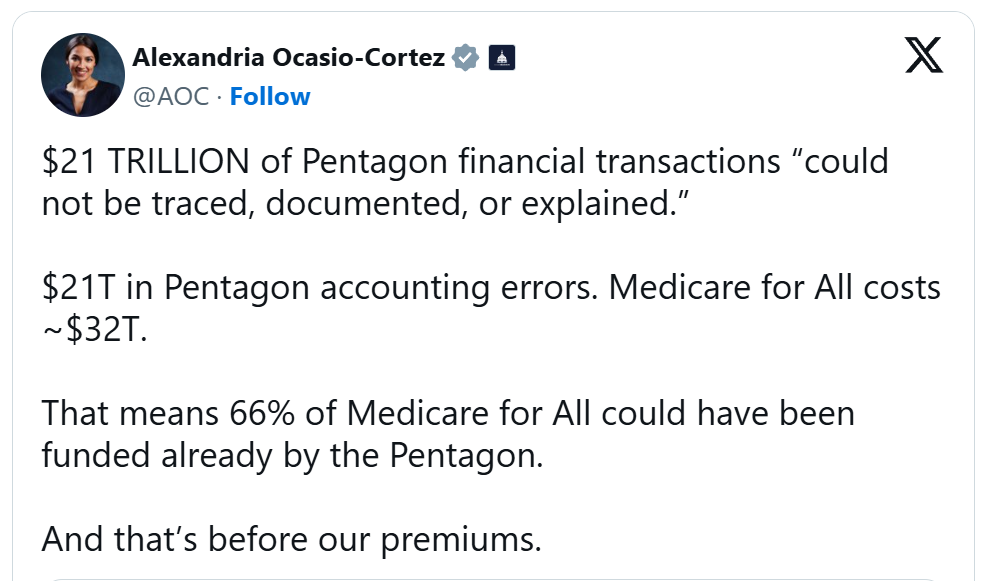
\includegraphics[height = .8\textheight]{AOC_tweet2.png}
\end{frame}



\begin{frame}
\frametitle{GDP}
\centering
\includegraphics[height = \textheight]{\graphdir gdpa_per_cap_log1870}
\end{frame}


\begin{frame}
\frametitle{Measuring GDP}
\begin{wideitemize}
\item Lots of things go into GDP
\begin{itemize}
\item Millions of Chickens
\item Billions of paperclips
\item Thousands of econ lectures
\end{itemize}
\item How do we add Apples and Oranges?
\end{wideitemize}

\end{frame}


\begin{frame}
\frametitle{Money}
\begin{wideitemize}
\item The natural metric for adding GDP is money prices.
\item Prices provide the relative value of things in an economy.
\item This turns out to be one of money'’s most important functions.
\end{wideitemize}
\end{frame}


\begin{frame}
\frametitle{Measuring GDP}
\begin{wideitemize}
\item Suppose that an economy had only two goods.
\begin{itemize}
\item Apples
\item Oranges
\end{itemize}
\item GDP in terms of prices would be

\begin{equation*}
GDP = (Q_A \times P_A) + (Q_O \times P_O)
\end{equation*}
\end{wideitemize}

\end{frame}


\begin{frame}
\frametitle{Measuring GDP}
\begin{wideitemize}
\item One way of measuring GDP would be to measure the price and quantity of everything sold in the country.

\item There is a second way -- we take advantage of circular flows in the economy.
\end{wideitemize}

\end{frame}


\begin{frame}
\frametitle{Measuring GDP}
\begin{wideitemize}
\item Imagine an economy with only one good, bread, produced using only labor.  There are two types of actors in this economy:

\begin{wideitemize}
\item Households
\begin{itemize}
\item Provide labor to make bread
\item Get paid wages by the firm (which they use to buy bread)
\end{itemize}
\item Firms
\begin{itemize}
\item Pay workers to make bread
\item Sell bread to households
\end{itemize}\end{wideitemize}
\end{wideitemize}
\end{frame}


\begin{frame}
\frametitle{Circular Flow Diagram (simple)}
\begin{columns}
\begin{column}{.5\textwidth}
\resizebox{\textwidth}{.5\textheight}{


\tikzset{every picture/.style={line width=0.75pt}} %set default line width to 0.75pt

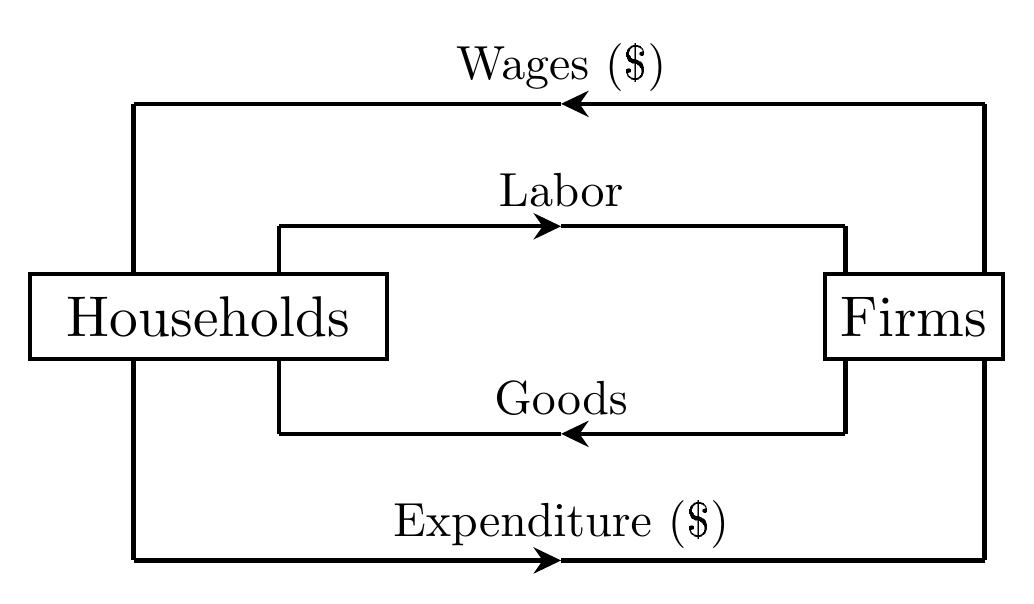
\begin{tikzpicture}[x=0.75pt,y=0.75pt,yscale=-1,xscale=1]
%uncomment if require: \path (0,300); %set diagram left start at 0, and has height of 300

%Straight Lines [id:da3142809335416301]
\draw [line width=1.5]    (124,59.5) -- (124,141) ;


%Straight Lines [id:da9626190695079444]
\draw [line width=1.5]    (124,182) -- (124,279.5) ;


%Straight Lines [id:da3345837970311947]
\draw [line width=1.5]    (124,279.5) -- (327,279.5) ;
\draw [shift={(330,279.5)}, rotate = 180] [fill={rgb, 255:red, 0; green, 0; blue, 0 }  ][line width=1.5]  [draw opacity=0] (13.4,-6.43) -- (0,0) -- (13.4,6.44) -- (8.9,0) -- cycle    ;

%Straight Lines [id:da01953277539539222]
\draw [line width=1.5]    (330,279.5) -- (534,279.5) ;


%Straight Lines [id:da7687846182646736]
\draw [line width=1.5]    (124,59.5) -- (330,59.5) ;


%Straight Lines [id:da44029552198348365]
\draw [line width=1.5]    (333,59.5) -- (534,59.5) ;

\draw [shift={(330,59.5)}, rotate = 0] [fill={rgb, 255:red, 0; green, 0; blue, 0 }  ][line width=1.5]  [draw opacity=0] (13.4,-6.43) -- (0,0) -- (13.4,6.44) -- (8.9,0) -- cycle    ;
%Straight Lines [id:da3663913301698425]
\draw [line width=1.5]    (534,59.5) -- (534,141) ;


%Straight Lines [id:da5032753193398922]
\draw [line width=1.5]    (534,182) -- (534,279.5) ;


%Straight Lines [id:da9932947895966895]
\draw [line width=1.5]    (194,182) -- (194,218.5) ;


%Straight Lines [id:da18539319752174643]
\draw [line width=1.5]    (194,118.5) -- (194,141) ;


%Straight Lines [id:da49775346522692754]
\draw [line width=1.5]    (194,118.5) -- (327,118.5) ;
\draw [shift={(330,118.5)}, rotate = 180] [fill={rgb, 255:red, 0; green, 0; blue, 0 }  ][line width=1.5]  [draw opacity=0] (13.4,-6.43) -- (0,0) -- (13.4,6.44) -- (8.9,0) -- cycle    ;

%Straight Lines [id:da34816473919309443]
\draw [line width=1.5]    (330,118.5) -- (467,118.5) ;


%Straight Lines [id:da1253109371352814]
\draw [line width=1.5]    (467,118.5) -- (467,141) ;


%Straight Lines [id:da5483581319301252]
\draw [line width=1.5]    (467,182) -- (467,218.5) ;


%Straight Lines [id:da11360523157716229]
\draw [line width=1.5]    (194,218.5) -- (330,218.5) ;


%Straight Lines [id:da04502522469810577]
\draw [line width=1.5]    (333,218.5) -- (467,218.5) ;

\draw [shift={(330,218.5)}, rotate = 0] [fill={rgb, 255:red, 0; green, 0; blue, 0 }  ][line width=1.5]  [draw opacity=0] (13.4,-6.43) -- (0,0) -- (13.4,6.44) -- (8.9,0) -- cycle    ;

% Text Node
\draw  [line width=1.5]   (74,141.5) -- (246,141.5) -- (246,182.5) -- (74,182.5) -- cycle  ;
\draw (160,162) node [scale=2.074] [align=left] {Households};
% Text Node
\draw  [line width=1.5]   (457,141.5) -- (543,141.5) -- (543,182.5) -- (457,182.5) -- cycle  ;
\draw (500,162) node [scale=2.074] [align=left] {Firms};
% Text Node
\draw (330,42) node [scale=1.7280000000000002] [align=left] {Wages (\$)};
% Text Node
\draw (330,101) node [scale=1.7280000000000002] [align=left] {Labor};
% Text Node
\draw (330,201) node [scale=1.7280000000000002] [align=left] {Goods};
% Text Node
\draw (330,262) node [scale=1.7280000000000002] [align=left] {Expenditure (\$)};


\end{tikzpicture}

}
\end{column}

\begin{column}{.5\textwidth}
\begin{wideitemize}
\item Households earn wages from firms.  All the income is in the form of wages.
\item Households spend all their income on goods.
\item GDP is both therefore both national income and national expenditure.
\end{wideitemize}
\end{column}
\end{columns}
\end{frame}




\begin{frame}
\frametitle{Complications in Counting GDP}
\begin{wideitemize}
\item Used Goods
\begin{wideitemize}
\item How do you count the sale of a used car?
\end{wideitemize}

\item Intermediate Goods
\begin{itemize}
\item Firm 1 makes Flour – sells it to Firm 2
\item Firm 2 makes bread – sells it to consumers
\item How do we count up GDP?
\end{itemize}
\end{wideitemize}
\end{frame}


\begin{frame}
\frametitle{Intermediate Goods}
\begin{wideitemize}
\item Adding up the value of flour and bread would be double counting.

\item We can fix this in two ways
\begin{itemize}
\item Just count final goods – in this case bread.
\item Add up the value added at each step; the value of the output minus the value of the inputs.
\end{itemize}
\end{wideitemize}
\end{frame}


\begin{frame}
\frametitle{Complications}
\begin{wideitemize}
\item Non-market goods
\begin{itemize}
\item Home cooked meals
\item Child care
\item Snow Shoveling
\end{itemize}
\item Imputed value
\begin{itemize}
\item Housing services
\item Government services
\end{itemize}
\end{wideitemize}

\end{frame}


\begin{frame}
\frametitle{Stocks vs. Flows}
\begin{wideitemize}
\item Think of a bathtub
\begin{itemize}
\item Stock – level of water in the tub at any time
\item Flow – quantity of water flowing in/out of the tub
\end{itemize}
\item Goods aren't produced instantly -– they are produced over time.
\begin{itemize}
\item We don't say a factory makes 100 loaves of bread, we say they make 100 loaves per day.
\end{itemize}
\end{wideitemize}
\end{frame}


\begin{frame}
\frametitle{Stocks vs. Flows}
\begin{wideitemize}
\item Stock -- quantity measured at any point in time.
\begin{itemize}
\item Credit Card Balance
\item Capital stock
\item Number of unemployed people

\end{itemize}
\item Flow -- Quantity measured per unit of time.
\begin{itemize}
\item Credit card charges/payments
\item Investment
\item Number of people losing their jobs
\end{itemize}
\end{wideitemize}
\end{frame}


\begin{frame}
\frametitle{Stocks vs flows == rates vs levels}
\centering
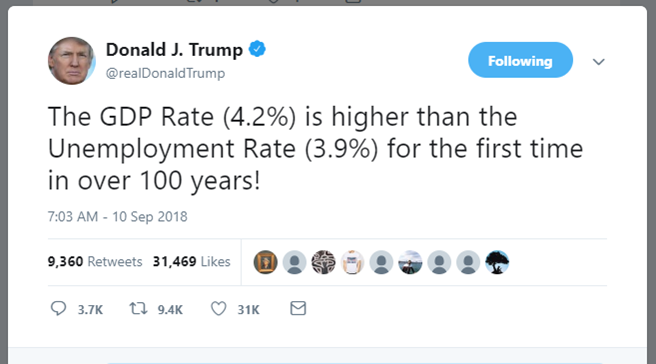
\includegraphics[height = .8\textheight]{trump_tweet.png}
\end{frame}

\begin{frame}
\frametitle{Components of GDP}
\begin{wideitemize}
\item There are four uses to which GDP can be put

\begin{equation*}
Y = C + I + G + NX
\end{equation*}

\item This is called the national income accounting identity.
\end{wideitemize}

\end{frame}


\begin{frame}
\frametitle{ Y = C + I + G + NX}

\begin{wideitemize}
\item C -- Consumption of goods and services by households.
\item I -- Investment.  Investment is anytime you buy something for use in the future.  Houses, factories.
\item G -- Government spending on goods and services -- like tanks and teachers.  Note that this does not include transfer payments.
\item NX -- Net exports.  This is the amount that we export, less the amount that we import.
\end{wideitemize}

\end{frame}


\begin{frame}
\frametitle{How large are the components?\\All values are annual nominal values for \lastyear}
\begin{center}
\begin{tabular}{|c|r|r|} \hline
Y & \$29.3T & Percent of GDP  \\ \hline
C & \$19.9T & 68\%\  \\ \hline
I & \$5.3T & 18\%\  \\ \hline
G & \$5.0T & 17\%\  \\ \hline
NX & -\$898B & -3\%\  \\ \hline
\end{tabular}
\end{center}

\end{frame}


\begin{frame}
\frametitle{Components over time - Consumption}
\centering
\includegraphics[height=\textheight]{\graphdir nipa_c_i_g_nx1945}
\end{frame}


\begin{frame}
\frametitle{Real GDP}
\begin{wideitemize}
\item Q:  Given our framework for calculating GDP, what would happen if prices doubled?

\item A:  Nominal GDP would double
\vspace{11pt}
\item Would this mean anything real?
\end{wideitemize}

\end{frame}


\begin{frame}
\frametitle{Real GDP}
\begin{wideitemize}
\item Since we want a measure of real stuff produced we need to filter out changes in prices.
\item We do this by using a uniform set of prices.
\end{wideitemize}

\end{frame}


\begin{frame}
\frametitle{Constructing Real GDP}
\begin{wideitemize}
\item Find the price of each good in a given base year.
\item Take the quantity of each good produced during the current year and multiply it by the price of that good in the base year.
\item Sum the value of all the goods produced.
\item Because the only thing changing over time is the quantity of goods, this gives us the changes in the quantity of stuff, irrespective of changes in prices.
\end{wideitemize}
\end{frame}


\begin{frame}
\frametitle{Real GDP - example}
\begin{wideitemize}
\item Suppose we want to construct RGDP in \thisyear \  using \baseyear \ as the base year.  In our economy with apples and oranges:
\begin{equation*}
RGDP_{\thisyear} = (Q_{A,\thisyearshort} \times P_{A,\baseyearshort})+(Q_{O,\thisyearshort} \times P_{O,\baseyearshort})
\end{equation*}
\item This gives us RGDP for \thisyear \  in \baseyear \ prices
\end{wideitemize}

\end{frame}


\begin{frame}
\frametitle{Real GDP}
\begin{wideitemize}
\item How would you calculate RGDP for \baseyear \ using \baseyear \ as the base year?
\end{wideitemize}

\end{frame}


\begin{frame}
\frametitle{Some numbers}
\begin{itemize}
\item Nominal GDP in \lastyear -- \$29.2 T
\item Nominal GDP in \baseyear -- \$19.6 T

\item Real GDP in \lastyear -- \$23.4 T (in \baseyear \$)
\item Real GDP in \baseyear -- \$19.6 T (in \baseyear \$)
\vspace{11pt}
\item The nominal increase was \$9.6 T
\item The real increase was \$3.8 T
\item The increase due to inflation was \$5.8 T
\end{itemize}

\end{frame}


\begin{frame}
\frametitle{The GDP deflator}

\begin{wideitemize}
\item Suppose that now we want to know how much prices have gone up.
\item There are two major price indices that we use.  One index is called the GDP deflator (also called the ``implicit price deflator for GDP'').
\end{wideitemize}
\begin{equation*}
GDPD = NGDP / RGDP
\end{equation*}
\end{frame}


\begin{frame}
\frametitle{The GDP deflator}

\begin{equation*}
GDPD = NGDP / RGDP
\end{equation*}

\begin{wideitemize}
\item For example, for \lastyear:
\begin{equation*}
GDPD = \frac{(Q_{A,\lastyearshort} \times P_{A,\lastyearshort})  +  (Q_{O,\lastyearshort} \times P_{O,\lastyearshort})}
{(Q_{A,\lastyearshort} \times P_{A,\baseyearshort})  +  (Q_{O,\lastyearshort} \times P_{O,\baseyearshort})}
\end{equation*}

\item Note that GDPD is 1 for the base year
\end{wideitemize}
\end{frame}


\begin{frame}
\frametitle{The GDP deflator - example}

\begin{wideitemize}
\item $NGDP_{\lastyearshort}$ = \$29.2 T
\item $RGDP_{\lastyearshort}$ = \$23.4 T (\baseyear\$)
\item $GDPD = NGDP/RGDP$ = 1.248
\item Prices rose by about 24.8\% between \baseyear \  and \lastyear
\end{wideitemize}
\end{frame}


\begin{frame}
\frametitle{Consumer Price Index (CPI)}

\begin{wideitemize}
\item The GDPD measures the prices of all the goods and services that are produced in the country.

\item What if we wanted to measure the price of a different bundle?
\begin{itemize}
\item Cost of being a Dartmouth student
\item Cost of being caffeinated for your 9am classes.
\end{itemize}
\end{wideitemize}
\end{frame}

\begin{frame}
\frametitle{Caffeine Price Index}
\begin{wideitemize}
\item Suppose you got data on the prices of coffee and tea.
\end{wideitemize}
\begin{wideitemize}
\item Q:  How much has the price of caffeine risen?
\end{wideitemize}
\begin{center}
\begin{tabular}{|l|l|l|} \hline
 & \lastyear & \thisyear  \\ \hline
Tea & 1.00 & 1.20  \\ \hline
Coffee & 1.00 & 1.40  \\ \hline
\end{tabular}
\end{center}
\end{frame}


\begin{frame}
\frametitle{Caffeine Price Index}
\begin{wideitemize}
\item A:  You can’t tell because you don't know how much to weight the two components.
\item We know that tea has gone up by 20\% and that coffee has gone up by 40\%.
\item Overall, the price of caffeinated beverages has gone up by somewhere between the two.  The overall change will be a weighted average.  But what weights to use?
\end{wideitemize}
\end{frame}

\begin{frame}
\frametitle{Caffeine Price Index}
\begin{wideitemize}
\item Suppose that we did a survey and found that in \lastyear \ (the base year), consumption of the two beverages was:

\begin{itemize}
\item Tea -- 1000 cups
\item Coffee -- 3000 cups
\end{itemize}
\item We can use these quantities as weights in our price index.  Coffee will have three times the weight of tea.
\end{wideitemize}
\end{frame}


\begin{frame}
\frametitle{Caffeine Price Index}
\begin{wideitemize}
\item Our caffeine consumption cost is:
\begin{wideitemize}
\item 1000 * 1.0 + 3000 * 1.0 = \$4,000 \ \ \ in \lastyear
\item 1000 * 1.2 + 3000 * 1.4 = \$5,400 \ \ \ in \thisyear
\end{wideitemize}
\item The price of caffeine had increased by 35\%.
\end{wideitemize}
\end{frame}


\begin{frame}
\frametitle{PNC Cost of Christmas}
\centering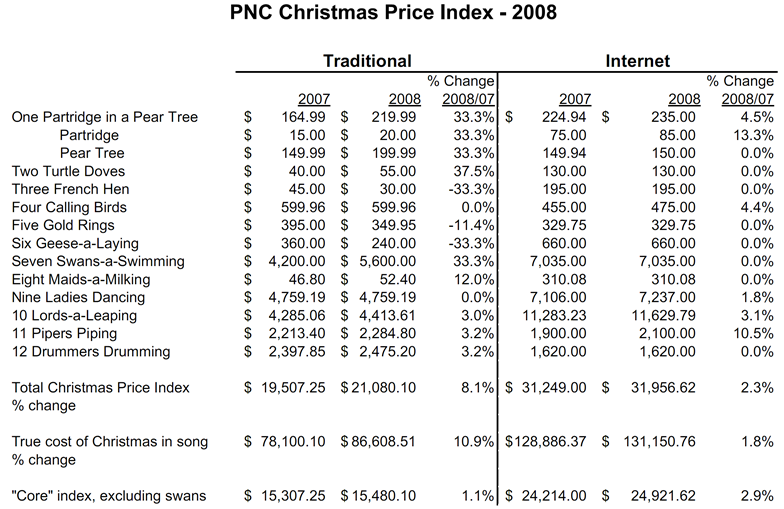
\includegraphics[height = .9\textheight]{PNC_12days.png}
\end{frame}


\begin{frame}
\frametitle{CPI -- Consumer Price Index}
\begin{wideitemize}
\item To calculate the CPI, you choose a base year and a basket of goods.
\item The CPI compares the cost of the basket today versus the cost in the base year.
\end{wideitemize}
\begin{equation*}
CPI_t = 100 \times\frac{\sum p_t \times q_{base}}{\sum p_{base} \times q_{base}}
\end{equation*}
\end{frame}


\begin{frame}
\frametitle{CPI}
\begin{wideitemize}
\item The basket of goods for the US is chosen by the government.
\item The government performs a survey to find out what people consume and in what proportions.  This determines the weights.
\end{wideitemize}
\end{frame}


\begin{frame}
\frametitle{Problems with the CPI}
\begin{wideitemize}
\item Suppose that you wanted to compensate people for the increased cost of their caffeine consumption.
\begin{wideitemize}
\item This is the idea behind cost of living adjustments (COLAs).
\end{wideitemize}
\item What if people only slightly prefer coffee to tea?
\end{wideitemize}
\end{frame}


\begin{frame}
\frametitle{CPI problems - Substitution}
\begin{wideitemize}
\item If people switch from coffee to tea, the increase in the price index overstates the needed increase in people's caffeine budgets.
\item If you increased everyone's caffeine budget by 35\% (the amount that the caffeine CPI has risen), they would be better off than they were before, because they are willing to switch to tea.
\end{wideitemize}
\end{frame}


\begin{frame}
\frametitle{CPI problems - Substitution}
\begin{wideitemize}
\item The problem with indexes based on a fixed basket of goods is it does not take account of the fact that people will switch from expensive products to cheaper ones.
\item This is an unavoidable problem with this sort of index.
\end{wideitemize}
\end{frame}



\begin{frame}
\frametitle{Differences between CPI and GDPD}
\begin{columns}[T]
\begin{column}{0.5\textwidth}
\begin{wideitemize}
\item CPI
\begin{itemize}
\item Basket of goods is just consumer goods
\item Goods produced abroad are counted
\item The basket of goods is from the base year (Laspeyres index, fixed basket)
\end{itemize}
\end{wideitemize}
\end{column}

\begin{column}{0.5\textwidth}
\begin{wideitemize}
\item GDPD
\begin{itemize}
\item Basket of goods is all goods
\item Goods produced abroad are not counted
\item The basket of goods is from the current year (Paasche index, changing basket)
\end{itemize}
\end{wideitemize}
\end{column}
\end{columns}
\end{frame}


\begin{frame}
\frametitle{Problems with choosing baskets}
\begin{wideitemize}
\item Suppose that we use a base year consumption basket from 50 years ago
\begin{wideitemize}
\item the typical basket that the average person got with the average salary.
\end{wideitemize}
\item Can we consume it now with an average salary?
\item Maybe, but some things have gone up tremendously in value, like land.
\end{wideitemize}
\end{frame}


\begin{frame}
\frametitle{Problems with choosing baskets}
\begin{wideitemize}
\item On the other hand, suppose that we use today's average consumption basket.
\item Could people in the past have consumed it with the average income?
\item No. we have things like iPhones, HDTV's and computers that they didn't have then, and other things are much cheaper now, like transatlantic transportation.
\end{wideitemize}
\end{frame}


\begin{frame}
\frametitle{CPI and GDPD}
\centering
\includegraphics[height = \textheight]{\graphdir inflation_cpi_gdpd1950}
\end{frame}


\begin{frame}
\frametitle{Unemployment}
\begin{wideitemize}
\item Perhaps the most watched economic statistic
\item Why?
\begin{itemize}
\item A well functioning economy uses all resources.  Unemployment wastes resources.
\item The costs are unevenly distributed
\end{itemize}
\end{wideitemize}
\end{frame}


\begin{frame}
\frametitle{Unemployment}
\centering
\includegraphics[height = \textheight]{\graphdir UR1995}
\end{frame}


\begin{frame}
\frametitle{Unemployment}
\begin{wideitemize}
\item To figure out unemployment, the government does a survey each month.
\item They divide the population into three groups.

\begin{equation*}
Adult \  population = (E + U) + OLF
\end{equation*}

\begin{itemize}
\item E -- employed
\item U -- unemployed
\item OLF -- out of labor force (students, retired, stay at home parents, etc.)
\end{itemize}
\end{wideitemize}
\end{frame}


\begin{frame}
\frametitle{Unemployment}
\begin{wideitemize}
\item The labor force consists of the Employed and the Unemployed
\begin{equation*}
LF = E + U
\end{equation*}
\item We can then form measures:
\begin{wideitemize}
\item Unemployment Rate
\end{wideitemize}
\begin{equation*}
UR = U / LF
\end{equation*}
\begin{wideitemize}
\item Labor force Participation Rate
\end{wideitemize}
\begin{equation*}
LFPR = LF/adult\  pop
\end{equation*}
\begin{wideitemize}
\item Employment to Population Ratio
\end{wideitemize}
\begin{equation*}
EPOP = E/adult\  pop
\end{equation*}

\end{wideitemize}

\end{frame}


\begin{frame}
\frametitle{Labor Force Size}
\centering
\includegraphics[height = \textheight]{\graphdir labor_force1998}
\end{frame}


\begin{frame}
\frametitle{Labor Force Participation Rate}
\centering
\includegraphics[height = \textheight]{\graphdir lfpr_1945}
\end{frame}


\begin{frame}
\frametitle{LFPR by Gender}
\centering
\includegraphics[height = \textheight]{\graphdir lfpr_both1945}
\end{frame}


\begin{frame}
\frametitle{Labor Force Participation Over the Business Cycle}
\centering
\includegraphics[height = \textheight]{\graphdir lfpr_1980}
\end{frame}


\begin{frame}
\frametitle{LSAT tests taken vs. Unemployment}
\centering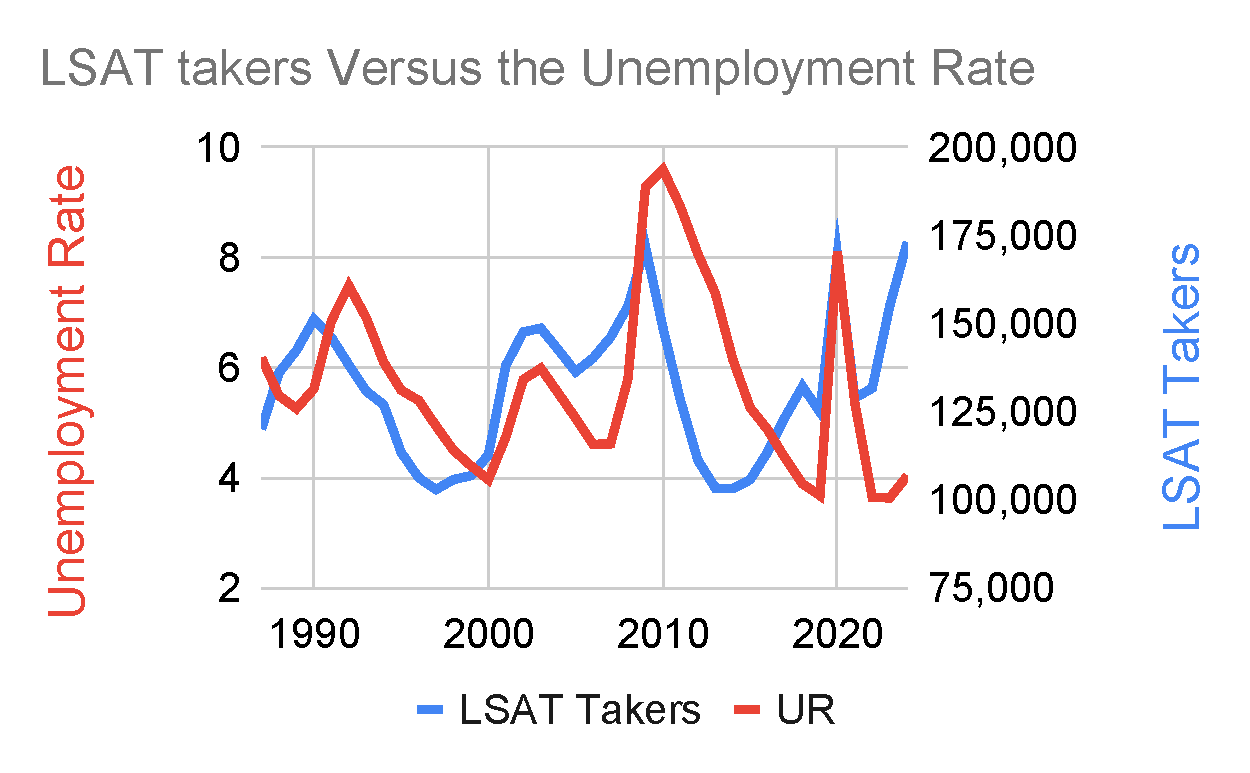
\includegraphics[height = \textheight]{LSAT2024.pdf}
\end{frame}


\begin{frame}
\frametitle{Seasonal Adjustments}
\centering
\includegraphics[height = \textheight]{\graphdir ur_season2005}
\end{frame}


\begin{frame}
\frametitle{Seasonal Adjustments}
\centering
\includegraphics[height = \textheight]{\graphdir ur_season2012}
\end{frame}


\begin{frame}
\frametitle{Size of Adjustments}
\centering
\includegraphics[height = \textheight]{\graphdir ur_season_adjustment2005}
\end{frame}


\begin{frame}
\frametitle{Okun’s Law}
\begin{wideitemize}
\item When unemployment is high, GDP growth tends to be low.
\begin{equation*}
Real \ GDP\ Growth =
3\% - 2 * \Delta Unemployment\ Rate
\end{equation*}
\item If the UR isn't changing, Real GDP growth is about 3\%.
\item For each percentage point increase in unemployment, real GDP growth declines by about 2%..
\end{wideitemize}
\end{frame}


\begin{frame}
\frametitle{Okun’s law}

\begin{equation*}
Real \ GDP\ Growth =
3\% - 2 * \Delta Unemployment\ Rate
\end{equation*}
\begin{wideitemize}\item To reduce unemployment by two percentage points the US needs to grow at about 7\%
\end{wideitemize}
\end{frame}


\begin{frame}
\frametitle{Okun's Law on Quarterly Data}
\centering
\includegraphics[height = \textheight]{\graphdir okun_quarterly}
\end{frame}


\begin{frame}
\frametitle{Okun's Law on Yearly Data}
\centering
\includegraphics[height = \textheight]{\graphdir okun_yearly}
\end{frame}


\begin{frame}
\frametitle{Okun’s Law Regression Results}
\begin{center}
\begin{tabular}{|lcc|} \hline
  & (1) & (2)  \\ 
VARIABLES & Yearly & Quarterly  \\ \hline
Change in Unemployment Rate & -1.50*** & -1.21***  \\ 
 & (0.13) & (0.06)  \\ 
Constant & 3.09*** & 0.78***  \\ 
 & (0.16) & (0.04)  \\ 
\hline
Observations & 74 & 310  \\ 
R-squared & 0.65 & 0.56  \\ \hline
\end{tabular}
\end{center}
\end{frame}

\end{document}
